%Recent efforts [cite Mizar, cite ACL2, cite Coq] have implemented the algorithm
%in proof assistants and formally proved claims about its behavior.
%However, because they operate entirely within idealized formal checkers,
%these works inadvertently gloss over certain classes of issues
%that routinely crop up in real-world settings.
\subsection{VST}
The Verified Software Toolchain is a separation-logic based software toolchain for C, allowing mechanized checking of user-provided proofs and specifications of C programs. Given a Coq-based proof that the C program matches the specification, VST guarantees the correctness of the verified program with the CompCert compiler~\cite{leroy:compcert}. The underlying logic behind the VST is Verifiable C, a subset of the CLight semantics provided by the CompCert compiler.

\subsubsection{Example of a specification}
\begin{lstlisting}
void initialise_list(int list[SIZE], int a) {
	for (int i = 0; i < SIZE; ++i) {
		list[i] = a;
	}
}
\end{lstlisting}
\begin{lstlisting}
Definition initialise_list_spec :=
DECLARE _initialise_list
WITH sh: share, arr : val, old_list: list val, a: Z
PRE [tptr tint, tint]
	PROP (
		writable_share sh;
		repable_signed a
	)
	PARAMS ( arr; Vint (Int.repr a) )
	GLOBALS ()
	SEP (
		data_at sh (tarray tint SIZE) (old_list) (arr)
	)
POST [ tvoid ]
	PROP ()
	LOCAL ()
	SEP (
		data_at sh (tarray tint SIZE) (list_repeat (Z.to_nat SIZE)
			(Vint (Int.repr a))) arr
	).
\end{lstlisting}
This is a sample VST \textit{function specification} of a C function \texttt{initialise\_list} defined above. The C implementation fills an input integer array of length \texttt{SIZE} with the integer \texttt{a}. We give a brief explanation of its structure.
\newline\newline
A C program is first run through CompCert's \textit{clightgen} utility to produce a Coq-based abstract syntax tree. VST uses this to allow us to write specifications like the example above. The \texttt{DECLARE} section matches the specification to the C function's name, while the \texttt{WITH} section quantifies the parameters in the specification. The \texttt{PRE} and \texttt{POST} sections describe the precondition and postcondition of the function. They commonly share a \texttt{PROP} and \texttt{SEP} subsection. \texttt{PROP} contains general propositions that are independent of the program state: in this case, that the user has writable access to the array, and the \texttt{a} to fill the array with is a 32-bit integer. \texttt{SEP} contains spatial assertions in VST's separation logic. In the precondition, one will also specify analogs of the actual C parameters, as well as any global variables used.
\newline\newline
Our task after writing the specification, is to provide a proof verifying that, if the function is called with the specified preconditions \textit{and} terminates successfully, then it returns the program state and propositions specified in the postcondition. Then, when verifying a program that \textit{calls} this function, one needs to prove that the program satisfies the preconditions of the function at the call, and in return receives the postcondition. This is how small verified functions can be built into larger programs in the VST.
\newline\newline
A full, technical explanation can be found in the VST's manual~\cite{vcmanual}.
\subsection{CertiGraph}

CertiGraph, previously known as RamifyCoq, is a library for reasoning about graphs and graph-manipulating C programs through the VST infrastructure. The bulk of the graph library is largely built in Coq, independent of the VST, but designed so that graphs can be represented in VST specifications and proofs.
\newline\newline
The workflow is as follows: we define a \textit{mathematical} model of the graph manipulated by a C program, then follow with \textit{spatial} representation lemmas of the graph - how the graph is represented in the program heap. Then, we write and prove VST specifications for the C program. The following diagram from Wang et al~\cite{DBLP:journals/pacmpl/WangCMH19} illustrates the relationship between CertiGraph and VST.
\newline\newline
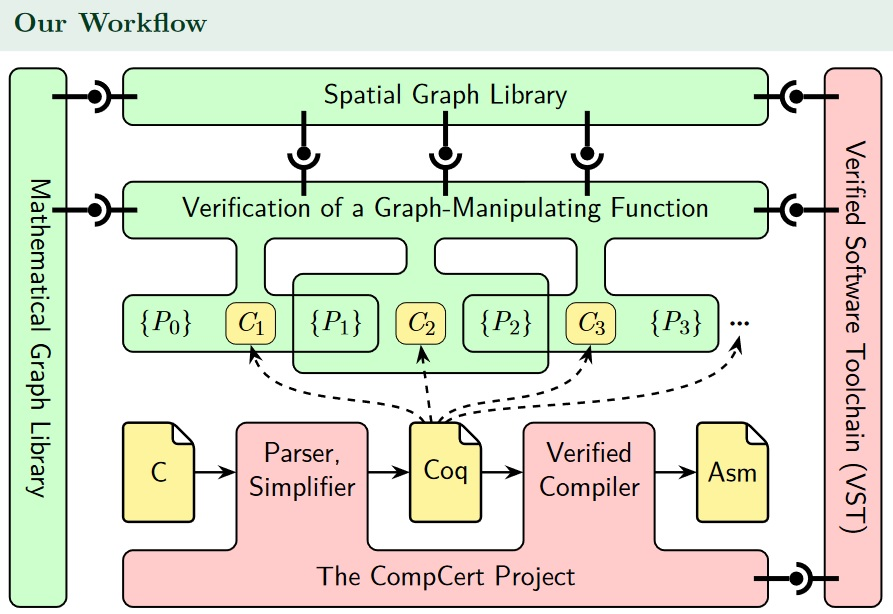
\includegraphics[scale=0.76]{certigraph_dep.jpg}
\newline\newline
The graph library has demonstrated its ability to verify C implementations of graph-related algorithms and data structures, including union-find, bipartition marking, and most significantly a garbage collector for the CertiCoq team~\cite{DBLP:journals/pacmpl/WangCMH19}.
\newline\newline
We performed a brief survey of similar work prior to this paper, listed under Section 6. Most of the existing work verify the algorithms wholly in the language of proof assistants. Very often, these languages are idealized and do not reason about issues such as overflow and pointer arithmetic. CertiGraph focuses on C implementations of these algorithms, reasoning about the proofs with Coq. It is more similar to Beckert and Furbach's approach to using KeY to verify Dijkstra's algorithm in C++ and Java~\cite{klasen2010verifying}. Because of our targeted language, we have to consider not only the graph algorithm's implementation, but also the spatial representation of graphs in C. These are not issues that need to be addressed by graphs and algorithms written in the language of the proof assistants.
\newline\newline
Ongoing work has been initiated by my research partner, Anshuman Mohan, to verify Dijkstra's algorithm~\cite{amdijkstra}. In the process, he discovered an integer overflow issue in the abstract algorithm, unhighlighted in functional implementations and proofs but meaningful in an actual C implementation. This highlights the value of our focus on C verification. I will make several references to the verification of Dijkstra's algorithm, as my work is a general extension of Anshuman's project.

\subsection{Contributions of this paper}

In this paper, I have further explored and verified two more common graph algorithms, Prim's and Kruskal's algorithms for generating a minimum spanning tree, with help from my partner, Anshuman Mohan. In the process, I have extended CertiGraph, a fundamentally directed graph library, to be able to reason about undirected graph properties. The verifications of these algorithms demonstrate the \textit{modular} nature of our graph library and VST verification, as we were able to make use of previous, independently verified C implementations and data structures. The verification of Prim's algorithm uncovered an observation that Prim's algorithm can return a forest for a disconnected graph in a single run, contrary to the common notion that Prim's algorithm by itself only returns trees.
\newline\newline
The verified code is available at \url{https://github.com/leowweixiang/CertiGraph}.